\documentclass[9pt,twocolumn]{extarticle}
\usepackage{amsmath}
\usepackage{graphicx}
\usepackage[margin=0.5in]{geometry}
\usepackage{listings}
\usepackage{wrapfig}
\usepackage{xcolor}

\lstdefinestyle{customc}{
  belowcaptionskip=1\baselineskip,
  breaklines=true,
  language=C,
  showstringspaces=false,
  basicstyle=\footnotesize\ttfamily,
  keywordstyle=\bfseries\color{green!40!black},
  commentstyle=\itshape\color{purple!40!black},
  identifierstyle=\color{blue},
  stringstyle=\color{orange},
}

\lstset{escapechar=@,style=customc}
\newcommand{\ttf}[1]{{\ttfamily #1}}

\begin{document}
\pagenumbering{gobble}
\section{Weak Memory Models}
\vspace{-0.25cm}
Programmers expect the actions of their imperative programs to execute in the order they define. Modern processor architectures may appear to ``reorder'' instructions for performance purposes. When a processor exhibits this type of behavior it is said to have a \textit{weak memory model}. Here we aim to help the programmer find bad behavior in concurrent algorithms due to weak memory models. The idea is to let the programmer manually reorder instructions and see the implications.

\vspace{-0.35cm}
\section{Baking Logistics}
\vspace{-0.25cm}

To build intuition for the effects of weak memory models we will use the analogy of a recipe (a program) and a baker (a process). For any recipe there are a list of steps to follow and with any luck the baker will produce the result defined by the recipe. Consider the example of a cake recipe (program): make the batter, make the icing, bake the cake, apply the icing.

Note, that the baker can safely swap the order of the first two tasks while preserving the result. This could be advantageous in the case where some ingredient required for the batter is not immediately available but everything necessary for making the icing is at hand. Similarly, it is sometimes advantageous for processors to reorder instructions for performance reasons.

Now imagine we introduce a second baker, but we also observe that the oven cannot accommodate more than one cake at a time. That is, if two cakes are cooked at the same time they will both be ruined. Further the bakers know from the recipe that if, when they go to get supplies for the icing, another baking pan is missing then someone is likely making a cake and they can't use the oven until that cake is done.

As defined, will the recipe guarantee that one cake or no cakes are in the oven at any given time? Does that hold if we swap the first two steps?

\vspace{-0.25cm}
\section{Concurrent Algorithms}
\vspace{-0.25cm}

\begin{figure}[h]
  \vspace{-0.6cm}
  \begin{minipage}{.24\textwidth}
        \lstinputlisting[
        xleftmargin=2.2em,
        xrightmargin=0em,
        framexleftmargin=1.5em,
        framexrightmargin=0em,
        numbers=left,
        numbersep=5pt,
        numberstyle=\scriptsize
        ]{code/dekker-p0.c}
  \end{minipage}
  \begin{minipage}{.25\textwidth}
        \lstinputlisting[
        xleftmargin=1em,
        xrightmargin=2.2em,
        framexleftmargin=0em,
        framexrightmargin=1.5em,
        numbers=left,
        numbersep=5pt,
        numberstyle=\scriptsize
        ]{code/dekker-p1.c}
      \end{minipage}
  \vspace{-0.25cm}
  \caption{Dekker's Mutex}
  \vspace{-0.25cm}
\end{figure}

The recipe, the ``pan-check'', and the two bakers are a useful approximation of a simplified version of Dekker's mutual exclusion algorithm (code above). The \ttf{flag0} and \ttf{flag1} are shared variables that each process \ttf{p0} and \ttf{p1} use to signal their intent to enter the critical section. The processes represent the bakers, setting the flags represent the procurement of a baking pan, checking the flags represents checking for a missing pan when making the icing, and the ``critical section'' represents the oven.

We can ask the same questions from above of Dekker's algorithm. If it executes as defined is it ever possible for both processes to enter the critical section? If not, will swapping store to \ttf{flag0} or \ttf{flag1} with the corresponding load of \ttf{flag1} and \ttf{flag0} make it possible for both processes to enter the critical section?

It turns out the answers are ``no'' and ``yes'', but the reasons why are not immediate.

\vspace{-0.25cm}
\section{Generating Examples}
\vspace{-0.25cm}
One way to determine whether swapping instructions will cause bad behavior is to find a bad execution. Doing this by hand plays out as follows: move one of the stores or loads around, try an execution for the instructions in each process, trace the result in your head, repeat steps two and three until you think you've exhausted the possible interleavings, start at step one.

We could also let the computer try all the possible permutations of the program following the steps we just outlined. This might work for Dekker's mutex but it's not clear this will scale well for more complex algorithms. More importantly computer generated counter examples might be hard to understand since the reason for arriving at a given counter example is partially opaque.

\vspace{-0.25cm}
\section{Instruction Scrub}
\vspace{-0.25cm}

Alternately we can provide tooling to see what happens when assignment to \ttf{flag0} in \ttf{p0} is allowed to reorder with the check of \ttf{flag1} which generates the following execution:

\vspace{0.25cm}
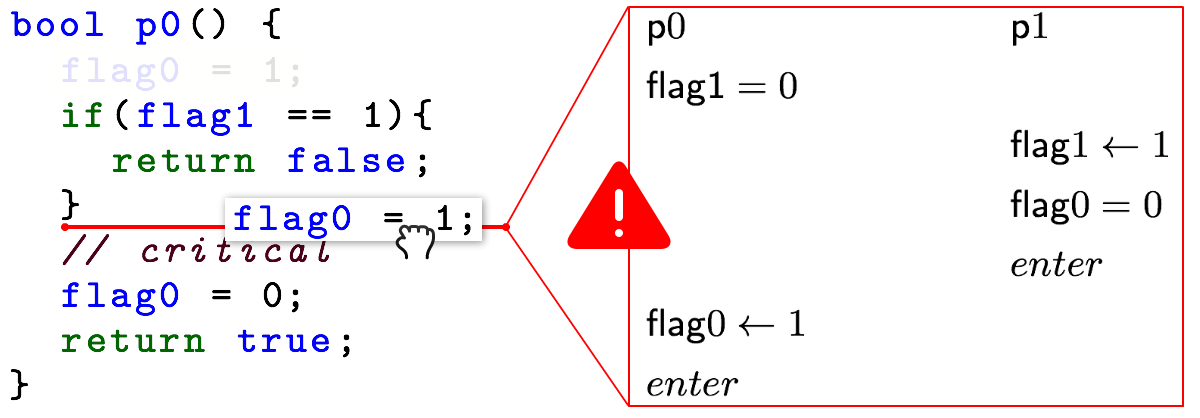
\includegraphics[width=0.45\textwidth]{images/scrub.png}
\vspace{0.25cm}

Interactive experimentation seems like a happy medium, especially if we just want to generate a bad execution. Based on what we know about the algorithm a good place to start moving things around is the store to \ttf{flag0} or \ttf{flag1}. Being able to ``grab'' the instructions and ``scrub'' them up and down the execution as illustrated while the computer checks for bad interleavings could mean quickly finding bad executions. Even if there is no specification. being able to view possible interleavings for bad state could still be valuable. Note that sifting through the possible executions will be necessary in this case.

The programmer provides the key insight about which instructions are most likely to be critical for correct execution and then the computer can quickly try executions as she moves the instructions around. This avoids the burden of having to figure out which instructions have side effects that we should be concerned about.

Also, viewing the side effects of the various executions and playing with the program state that results tells the programmer about the algorithm and how it will behave under a given weak memory model. This is true even if no ``bad'' executions are found.

\vspace{-0.25cm}
\section{Drawbacks}
\vspace{-0.25cm}

This technique is made awkward by the requirement to provide or define the processes so that executions can be examined or displayed to the user. It's possible to infer them from the points at which a program forks off threads (e.g. \ttf{pthread\_create}). Threads created in loops might have to simplified to just the case of two threads to avoid information overload.

There is also a distinction between the lines of code in C/C++ and the machine level instructions. The mapping can be retained using debugging information but helping the user identify the mapping between the code on the left and the bad execution of instructions on the right might be difficult or hard to understand.

\vspace{-0.25cm}
\section{Further Ideas}
\vspace{-0.25cm}

Assuming some mechanism for tracking shared state access, a language-IDE combination could overlay all the possible points at which a given instruction could move to within the existing source if it's movement might be problematic. This might provide an early warning about undesirable behavior.

\vspace{-0.25cm}
\section{Conclusion}
\vspace{-0.25cm}

It seems like tooling and language support could provide meaningful aid to concurrent algorithm designers working with (or without!) weak memory models in mind.
\end{document}